% !TeX root = ../thuthesis-example.tex

\chapter{SUMMARY, DISCUSSION AND FUTURE DIRECTIONS}

\section{Discussion and future directions}

Оригинальность работы состоит в том, что не существует исследований на тему создания и взаимодействия устройств для VR-IoT окружения, все исследователя концентрируются именно на управлении IoT устройствами с помощью шлемов виртуальной реальности.
Автор надеется продолжить работу над платформой в будущем уже в лаборатории университета. Остановимся подробнее на дальнейших этапах разработки, предложенных автором.

\begin{figure}
  \centering
  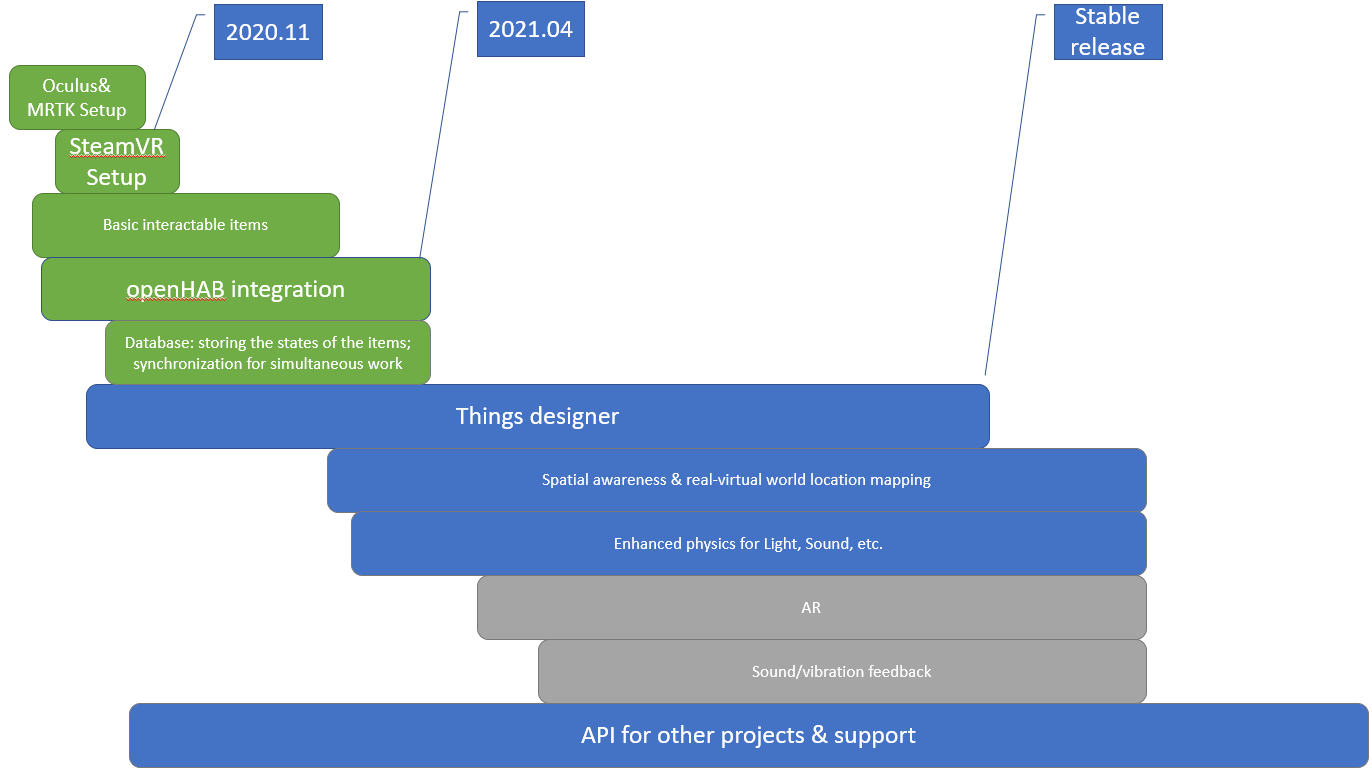
\includegraphics[width=0.9\linewidth]{figures/Timeline.png}
  \caption{Timeline}
  \label{fig:Timeline-figure}
\end{figure}

As seen in (Figure~\ref{fig:Timeline-figure}), the development started from providing support for Virtual reality headsets. Следующий шагом была реализация поддержки openHAB и базы данных для одновременной работы в одной среде. В тексте данной работы обсуждалось, что данные две задачи можно считать выполненными. Тем не менее, разработку Things designer пока на данный момент считать завершенной нельзя, так как необходимо дальнейшее исследование, to provide a bigger variety of supported Widgets and Items.

Mixed Reality toolkit can provide real-world environmental awareness for apps running on Hololens. It is already possible to run NUIX-Studio APP on Hololens, although, it has not yet been tested. Using spatial awareness, it will be possible to align virtual Widgets onto IoT devices. Developing real-virtual world location mapping for the Widgets for Virtual reality will be needed as well.

Currently, only advanced illumination can be computed on the NUIX-Studio APP. Researchers may need more accurate data to create new IoT devices. In this case Unity Game Engine can be extended with more accurate light, sound and other physics support.

Providing AR support requires adding new interactions techniques, as well as training Deep learning models to provide object recognition. Researchers can use both AR and VR to research on new IoT devices, with AR being responsible for retrieving the coordinates of the devices from the real world (by OpenCV, Tensoflow Graphics, etc.), and VR for visualizing environments that are difficult or impossible to show in AR (for example, flying on a plane or driving a car).

Augmented reality, Virtual reality and Mixed Reality are not the only interfaces to interact with IoT. What if the feedback from IoT devices only by sound and vibrations is provided? NUIX-Studio can be adapted for such limitations. One of the example usages of this approach is a research for visually impaired people in IoT environment.

Во время всего цикла разработки должен разрабатываться API для встраивания внешних разработок в платформу, в том числе проектов студентов HCI Lab.

\section{Summary}

Цель работы выполнена: представлена платформа для создания новых устройств для существующего IoT мира в виртуальной реальности, помогающая создавать новые устройства. Показано, что она позволяет это выполнить как теоретически, так и практически.
